% Copyright (C)  2015  Alexander Jankowski, Philipp Hacker.
% Permission is granted to copy, distribute and/or modify this document
% under the terms of the GNU Free Documentation License, Version 1.3
% or any later version published by the Free Software Foundation;
% with no Invariant Sections, no Front-Cover Texts, and no Back-Cover Texts.
% The lincense itself can be found at <https://www.gnu.org/licenses/fdl-1.3>.

\documentclass[numbers=noenddot,a4paper,notitlepage,twoside,BCOR15mm]{scrartcl}
%\documentclass[numbers=noenddot,12pt,a4paper]{scrartcl}

\usepackage{ifoddpage}
\usepackage[infoshow]{tabularx}
\usepackage{fancyhdr}
\usepackage[greek,ngerman]{babel}
\usepackage[T1]{fontenc}
\usepackage[utf8]{inputenc}
\usepackage{libertine}
\usepackage{ziffer}
\usepackage{graphicx}
\usepackage{units}
\usepackage[infoshow]{tabularx}
\usepackage[all]{xy}
\usepackage{amsmath}
\usepackage{amssymb}
\usepackage{wrapfig}
\usepackage{upgreek}
\usepackage{esint}
\usepackage{float}
\usepackage[font=small,labelfont=bf]{caption}
\usepackage{subcaption}
\usepackage{lscape}
\usepackage[backref=page]{hyperref}
\usepackage{cleveref}
\usepackage{csquotes}

\renewcommand{\headrulewidth}{0.1pt}
\renewcommand{\footrulewidth}{0.1pt}
\newcommand{\name}{\text{Name}} %TODO Name des Protokollanten eintragen

\renewcaptionname{ngerman}{\figurename}{Abb. }
\renewcaptionname{ngerman}{\tablename}{Tab.}

\setlength{\parindent}{0pt}

\newcommand{\nummat}[1]{\left[\text{#1}\right]}
\newcommand{\num}[1]{$\left[\text{#1}\right]$}
\newcommand{\degree}{^\circ}
\newcommand{\diff}{\textnormal{d}}
\newcommand{\tenpo}[1]{ 10^{#1}}
\newcommand{\greek}[1]{\greektext#1\latintext}
\newcommand{\ix}[1]{_\text{#1}}
\newcommand{\imag}{\mathbf{i}}
\newcommand{\tilt}[1]{\textit{#1}}
\newcommand{\grad}[1]{\textit{grad}\left(#1\right)}
\newcommand{\divergenz}[1]{\textit{div}\left(#1\right)}
\newcommand{\euler}{\mathnormal{e}}
\newcommand{\fett}[1]{\textbf{#1}}
\newcommand{\einnup}{\hspace{0.2cm}}
\newcommand{\einnum}{\hspace{-0.2cm}}
\newcommand{\zentriert}[1]{\begin{center}#1\end{center}}

\title{Protokoll: Paul-Fallen} %TODO Name des Versuchs eintragen
\author{Alexander Jankowski, Philipp Hacker}
\date{\today}
\pagestyle{fancy}
\fancyhead[C]{\thepage}
\fancyhead[R]{\name}
\fancyfoot[C]{\thepage}
\fancyhead[L]{Abschnitt \thesection}

\begin{document}
	\maketitle
	\begin{center}
		Betreuer: Dirk Weidermann \\ %TODO Name des Betreuers eintragen
		Versuchsdatum: 25.11.2015\\ %TODO Datum des Versuchs eintragen
		\begin{table}[h]
			\centering
			Note: %TODO Gute Note erhalten :)
			\begin{tabularx}{1.5cm}{|X|}
				\hline \\ \\
				\hline
			\end{tabularx}
		\end{table}
	\end{center}
	\vspace*{\fill}
	\tableofcontents
	\vfill
	\newpage
	\section{Motivation}
	Ionenfallen und insbesondere Paulfallen sind wichtige Werkzeuge der modernen Atom-, Molekül- und Clusterphysik. Sie werden benutzt für Anwendungen wie Massenspektrometrie, Speicherung und Manipulation von Nanoteilchen. Ohne das Prinzip einer Ionenfalle wäre es in der modernen Physik kaum möglich Nanoteilchen zu untersuchen. In ihnen können Teilchen, je nach Bauart beispielsweise über lange Zeiten oder große Massenbereiche gespeichert und im Vakuum untersucht werden. Die hyperbolische Paulfalle hast z.B. den Vorteil gegenüber linearen Paulfallen und Penningfallen, das diese geladene mit verschieden Ladungsvorzeichen speichern kann. Zur Untersuchung der gespeicherten Ionen können weiterhin ein weitreichendes Spektrum von Methoden angewandt werden, wie z.B. die Untersuchung von Stößen mit Puffergas, die Anregung der Ionen durch externe elektrische Wechselspannungsfelder oder Flugzeit-Massen-Spektrometrie, wodurch eine Vielzahl von physikalischen Eigenschaften der Ionen mit Hilfe von Ionenfallen untersucht werden können.
	\newpage
	\section{Physikalische Grundlagen}
	
	Im allgemeinen Fall werden Paulfallen als eine Anordnung von radialsymmetrischen Elektroden beschrieben, welche durch anlegen von Wechselspannung die Bewegung von Ionen auf ein begrenztes Volumen beschränkt. Für diese Beschränkung wird angenommen, dass Ionen, welche sich von dem Fallenzentrum entfernen eine lineare rücktreibende Kraft
	\begin{equation}
		\vec{F} \propto -\vec{r}
	\end{equation} 
	erfahren. Durch diese Annahme ergibt sich für die Falle ein harmonisches Speicherpotential
	\begin{equation}
		\Phi(x,y,z) = \Phi_0 \left(ax^2+by^2+cz^2\right),
	\end{equation}
	in welchem die Bewegungsfrequenzen der Ionen unabhängig von ihrer Position und Geschwindigkeit sind. Dieses Potential genügt der Laplace-Gleichung
	\begin{equation}
		\Delta \Phi(\vec{r}) = 0,
	\end{equation}
	solange die Bedingung für die Koeffizienten
	\begin{equation}
		a+b+c = 0
	\end{equation}
	erfüllt ist. In diesem Versuch wird eine hyperbolische Paulfalle betrachtet, was eine Lösung für die Koeffizienten
	\begin{equation}
		a = b \,\,\text{und}\,\, c = -2a
	\end{equation}
	vorgibt. Bei der hyperbolischen Falle sind die Endkappen bzw. der Elektrodenring wie Äquipotentialflächen geformt (vgl. Abb. \ref{img:schem_aufbau}). Um die Größe der Falle zu dimensionieren wird ein weiterer Parameter
	\begin{equation}
		d_0^2 = \frac{r_0^2}{2}+z_0^2
	\end{equation}
		\begin{figure}[t]
			\centering
			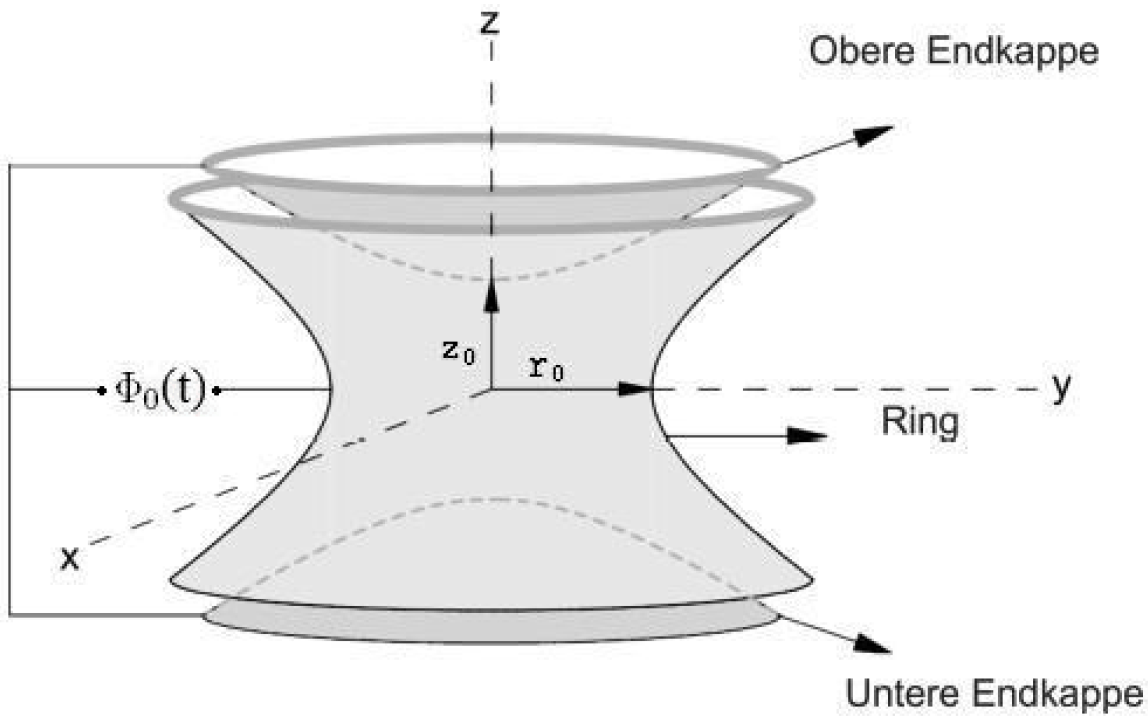
\includegraphics[width=0.6\textwidth]{pics/paul_schema.png}
			\caption{Schematischer Aufbau einer Paul-Falle mit radialsymmetrischer Geometrie. Hyperbolische Formen als Äquipotentialflächen. \cite{EMAUGreifswaldPaul}}\label{img:schem_aufbau}
		\end{figure}
	definiert, wobei $r_0$ und $z_0$ der minimale Abstand zur Ringelektrode bzw. den Endkappenelektroden sind. Weiterhin wird angenommen, dass sich die Amplitude des Potential aus einem Gleichspannungsanteil $U_0$ und einem Wechselspannungsanteil $V_0$ ergibt. Daraus folgt
	\begin{equation}
		\Phi_0 = U_0 + V_0\cdot \cos(\Omega t).
	\end{equation}
	Hierbei ist $\Omega$ die Führungsfeldfrequenz. Mit diesen Definitionen ergibt sich das gesamte Potential zu
	\begin{equation}
		\Phi(x,y,z,t) = \frac{U_0+V_0 \cdot \cos(\Omega t)}{2 d_0^2}\left(x^2+y^2-2z^2\right).
	\end{equation}
	Aus diesem Potential ergibt sich die Bewegungsgleichung
	\begin{equation}
		m\ddot{\vec{\eta}} = -Q \cdot \vec{\nabla} \Phi_\eta \,\,\text{mit}\,\, \eta=x,y,z
	\end{equation}
	eines Ions mit der Ladung $Q$ und der Masse $m$ zu
	\begin{align}
	\label{eq:BWGL}
		0 =& \frac{d^2}{dt^2} \begin{pmatrix} x \\ y \end{pmatrix} +\frac{Q}{md^2_0}(U_0 + V_0\cos(\Omega t))\begin{pmatrix} x \\ y \end{pmatrix} \nonumber \\
		0 =& \frac{d^2}{dt^2} z -\frac{2Q}{md^2_0}(U_0 + V_0\cos(\Omega t))z
	\end{align}
	Zur Lösung dieses Differentialgleichungssystems werden zunächst die Parameter
	\begin{align}
		\label{eq:Parameter}
		\tau =& \frac{1}{2}\Omega t, \nonumber \\
		a_z =& -2a_x = -2a_y = -\frac{8QU_0}{md_0^2\Omega^2}\,\,\text{und} \\
		q_z =& -2q_x = -2q_y = \frac{4QV_0}{md_0^2\Omega^2} \nonumber
	\end{align}
	definiert und die Gleichungen \eqref{eq:BWGL} können überführt werden in die kanonische Form der Mathieuschen Differentialgleichung:
	\begin{equation}
		0 = \frac{d^2\eta}{d\tau^2}+\left(a_\eta-2q_\eta \cos\left(2\tau \right)\right).
	\end{equation}
	Durch ausführliche Betrachtung der Lösung dieser Gleichung kann ein Stabilitätsparameter $\beta_\eta$ definiert werden, welcher in Abhängigkeit von $a_\eta$ und $q_\eta$ implizit als Kettenbruch ausgedrückt werden kann. Als vereinfachte Näherung gilt für kleine Parameter $a_\eta$ und $q_\eta$
	\begin{equation}
		\beta_\eta^2 = a_\eta - \frac{\left(a_\eta - 1\right)q_\eta^2}{2\left(a_\eta -1\right)^2-q_\eta^2}-\frac{(5a_\eta+7)q_\eta^4}{32(a_\eta-1)^3(a_\eta-4)}-\frac{(9a_\eta+58a_\eta+29)q_\eta^6}{64(a_\eta-1)^5(a_\eta-4)(a_\eta-9)}.
	\end{equation}
	Für einen Parameterwert im Intervall $\beta_\eta\,\epsilon\,(0,1)$ gilt, dass das betrachtete Ion in dieser Richtung $\eta$ eine beschränkte Bewegung vollführt und somit gespeichert ist. Da dies für alle drei Raumrichtungen gelten soll, müssen die Parameter der Falle $a$ und $q$ entsprechend gewählt werden. Da die Parameter für die verschiedenen Richtungen nach \eqref{eq:Parameter} zusammenhängen, kann ein sogenanntes Stabilitätsdiagramm angefertigt werden, dessen Form nicht mehr abhängig ist von den direkten physikalischen Parametern der Falle, sondern nur noch von $a_z$, $q_z$ und der Symmetrie der Falle. Für einen hyperbolischen Aufbau erhält man ein Diagramm nach Abb.\ref{img:stab1}. Wird jedoch die Rücktransformation der Parameter auf die Größen $U_0$ und $V_0$ betrachtet, so skaliert die Größe des Stabilitätsbereiches mit der Masse $m$.\\
		\begin{figure}[t]
			\centering
			\begin{subfigure}[t]{0.4\textwidth}
				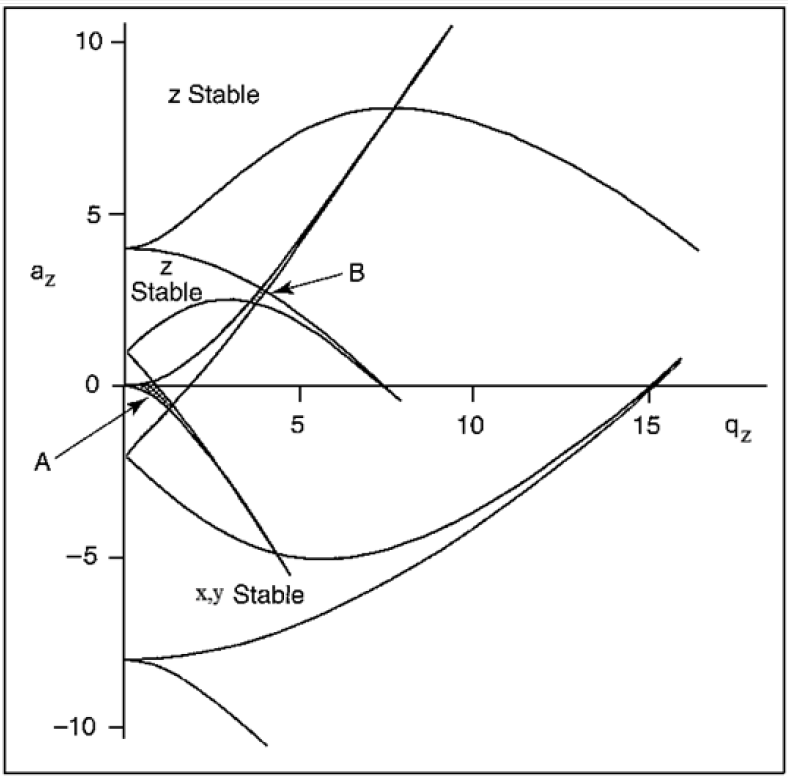
\includegraphics[width=\textwidth]{pics/stab_1.png}
				\caption{}\label{img:stab1}
			\end{subfigure}
			\vspace{0.2cm}
			\begin{subfigure}[t]{0.37\textwidth}
				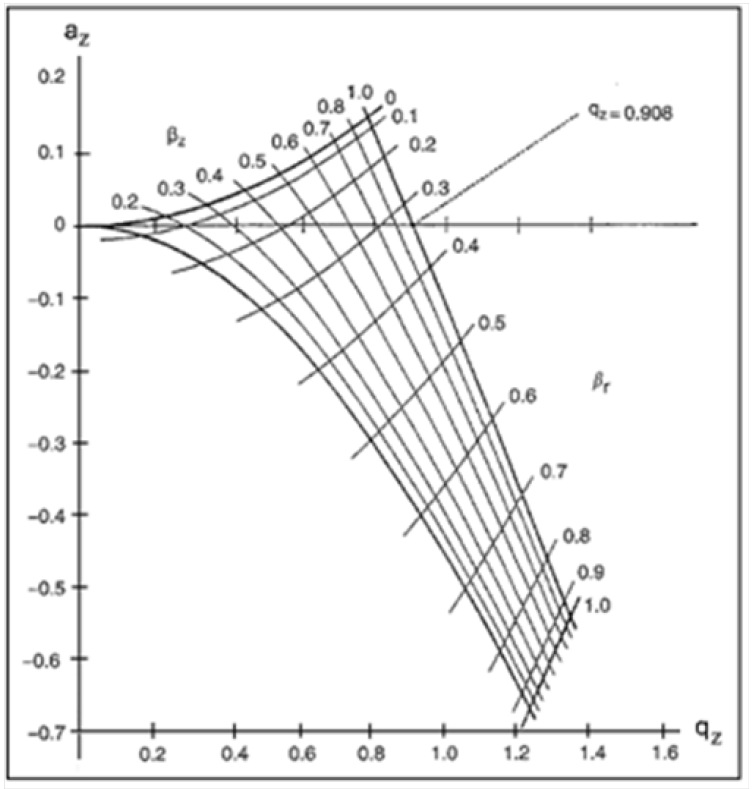
\includegraphics[width=\textwidth]{pics/stab_2.png}
				\caption{}\label{img:stab2}
			\end{subfigure}
			\caption{\fett{(a):} $a\ix{z}$ gegen $q\ix{z}$. Überlappungen der Graphen sind Gebiete dreidimensionaler Speicherung. \fett{(b):} Vergrößerung des Bereiches A aus \fett{(a)}. Eingezeichnet sind die Linien gleichen $\beta\ix{z}$ und $\beta\ix{r}$. }\label{img:stab}
		\end{figure}
		\begin{figure}[!h]
			\centering
			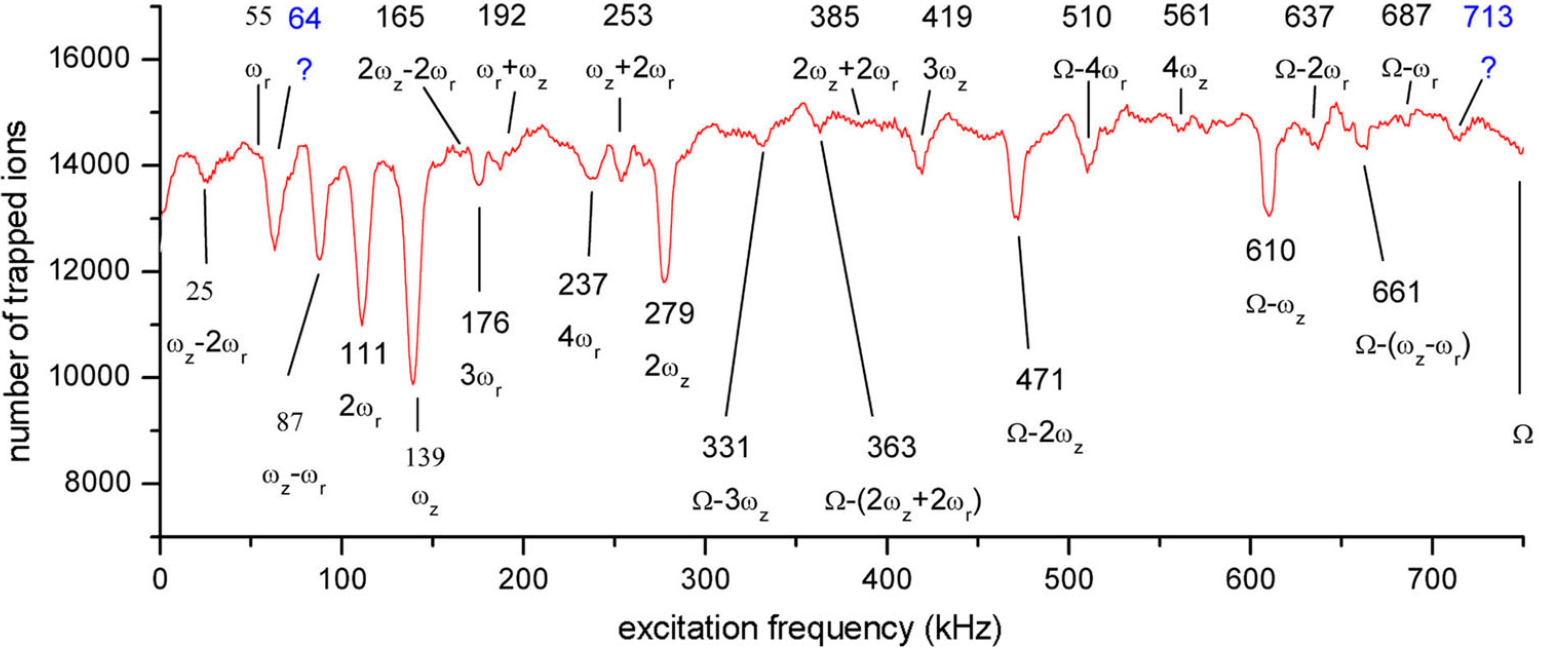
\includegraphics[width=\textwidth]{pics/referenz.png}
			\caption{Literatur-Spektrum aus \cite{Paul-FalleREF} für $\fett{N}_2$-Ionen. Angetragen sind die jeweiligen Resonanzfrequenzen für die Differenz aus Signalen einer Referenz ohne und mit Anregung.}\label{img:referenz}
		\end{figure}
	Aus der Lösung der Mathieuschen Differentialgleichungen lassen sich weiterhin die Bewegungsfrequenzen der Ionen bestimmen. Diese sind für kleine $a_\eta$- und $q_\eta$-Parameter bestimmt durch
	\begin{equation}
		\omega_{n,\eta} = \frac{(2n\pm \beta_\eta)\Omega}{2}.
	\end{equation}
	Die Kenntnis dieser Frequenzen ermöglicht es ein Ion in einer Paulfalle resonant anzuregen und damit diese aus der Falle zu extrahieren.

	\newpage
	\section{Durchführung}
	In diesem Versuch wird eine hyperbolische Paulfalle mit einem Fallenparameter von $d_0 = 7\,\mathrm{mm}$ verwendet, welche in einem Vakuumaufbau schematisch nach Abb.\ref{img:aufbau} aufgebaut ist. Die Ringelektrode ist in vier Elektroden segmentiert und die Endkappen besitzen zentrale Bohrungen, wodurch Elektronen eingelassen bzw. Ionen ausgeworfen werden können. Der Druck im Fallenbereich befindet sich während den Messungen in einen Bereich von $10^{-7}\,\mathrm{mbar}$. Über ein Ventil wird N$_2$-Gas in die Falle eingelassen, welches ionisiert und in der Falle gespeichert wird. Zur Ionisation wird eine Elektronenkanone verwendet, welche einen $95\,\mathrm{eV}$ Elektronenstrahl axial durch die Falle schickt, wo diese durch Elektronenstoßionisation N$_2^+$-Ionen erzeugen. Diese können bei den gegebenen Parametern der Führungsfeldfrequenz $\Omega = 1,29\,\mathrm{MHz}$ und einer Wechselspannungsamplitude $V_0  = 240\,\mathrm{V_{pp}}$ gespeichert werden können. Für die Extraktion der Ionen aus der Falle ist ein Funktionsgenerator an die Endkappen angeschlossen, welcher ein Sinus-Signal der Frequenz $\omega_z = 350\,\mathrm{kHz}$ bei kleinen Spannungsamplituden $\leq 5\,\mathrm{V}$ erzeugen kann. Durch diese Anregung werden die Ionen axial beidseitig aus der Falle getrieben. Auf der einen Seite befindet sich ein Channeltron-Detektor auf dem die Ionen detektiert werden können. Dieser wird mit einer Detektorspannung von $-2,4\,\mathrm{kV}$ und einer Dynodenspannung von $-4,5\,\mathrm{kV}$ betrieben. Die Messung wird über einen PC mit einer Kontrollsoftware gesteuert und mit Hilfe einer Datenkarte werden die Messungen aufgezeichnet. Jede individuelle Messung wird mehrfach durchgeführt, um viele Daten zu akkumulieren und den Einfluss statistischer Schwankungen zu minimieren.
		\begin{figure}
			\centering
			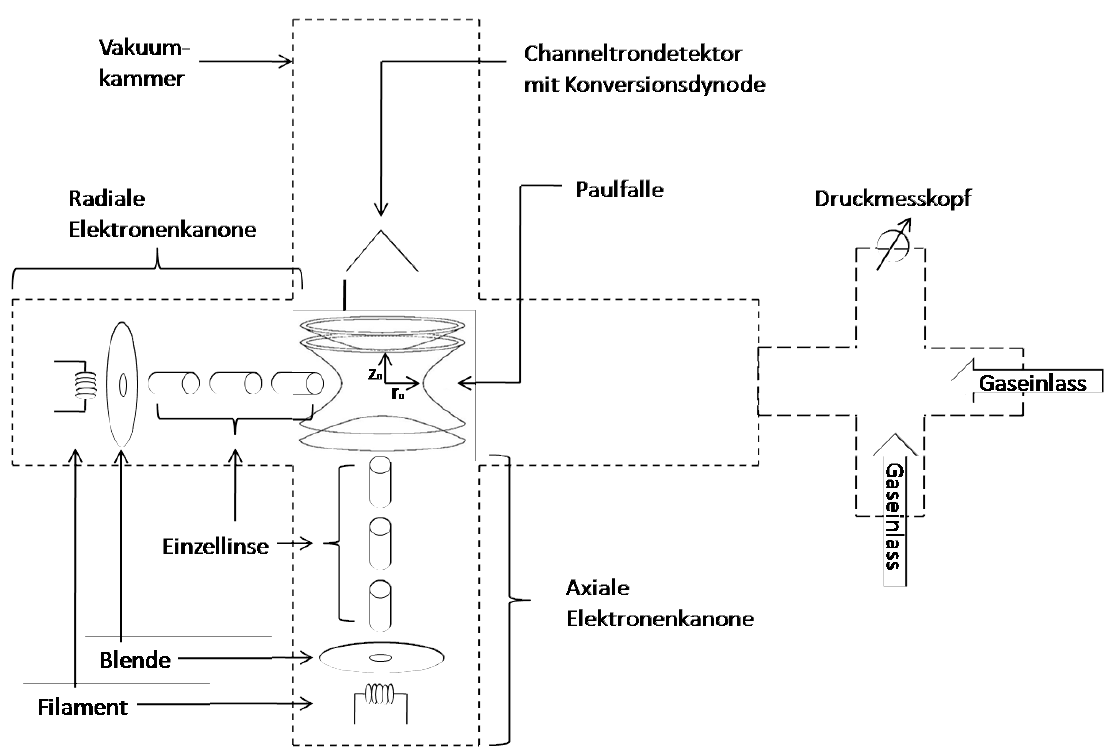
\includegraphics[width=1\textwidth]{pics/aufbau.png}
			\caption{Schematischer Aufbau des Versuchs. \cite{EMAUGreifswaldPaul}}\label{img:aufbau}
		\end{figure}

	
	
	\newpage
		\section{Auswertung}
		
		\subsection{Variation der Speicherzeit}
		
		Nachdem man sich mit dem Aufbau und der dazugehörigen Steuerung vertraut gemacht hatte, wurde ein Scan für die Speicherzeit in der Falle durchgeführt. Das heißt, dass die Zeit zwischen Ionisation (Elektronenkanone an) und Auswurf-Anregung durch den ersten Manipulationsgenerator variiert wurde. Die Ergebnisse sind in \autoref{img:zeit} zu sehen. Zu erwarten ist ein exponentielle Zusammenhang nach \tilt{Lambert-Beer}, da die kollektive Ionenbewegung und die Lebensdauerverteilung statistisch sind. Eine logarithmische Auftragung liefert die Bestätigung mit \autoref{img:lin}. Die 'Lebensdauer' bzw. die mittlere Verweildauer in der Falle bestimmte sich zu $\unit[5,1408]{ms}$.\\
		Eine Einzelmessung bestand jeweils als 10 'inneren' Iterationen, d.h. Messzyklen, welche in ihrer Intensität aufsummiert wurden. 50 äußere Iteration wiederholen den gesamten Vorgang von einer Wartezeit 0 bis $\unit[500]{\mu s}$ in chronologischer Reihenfolge, um eventuelle Zeitabhängige Fehler in der Messung zu eliminieren.
		
		\begin{figure}
			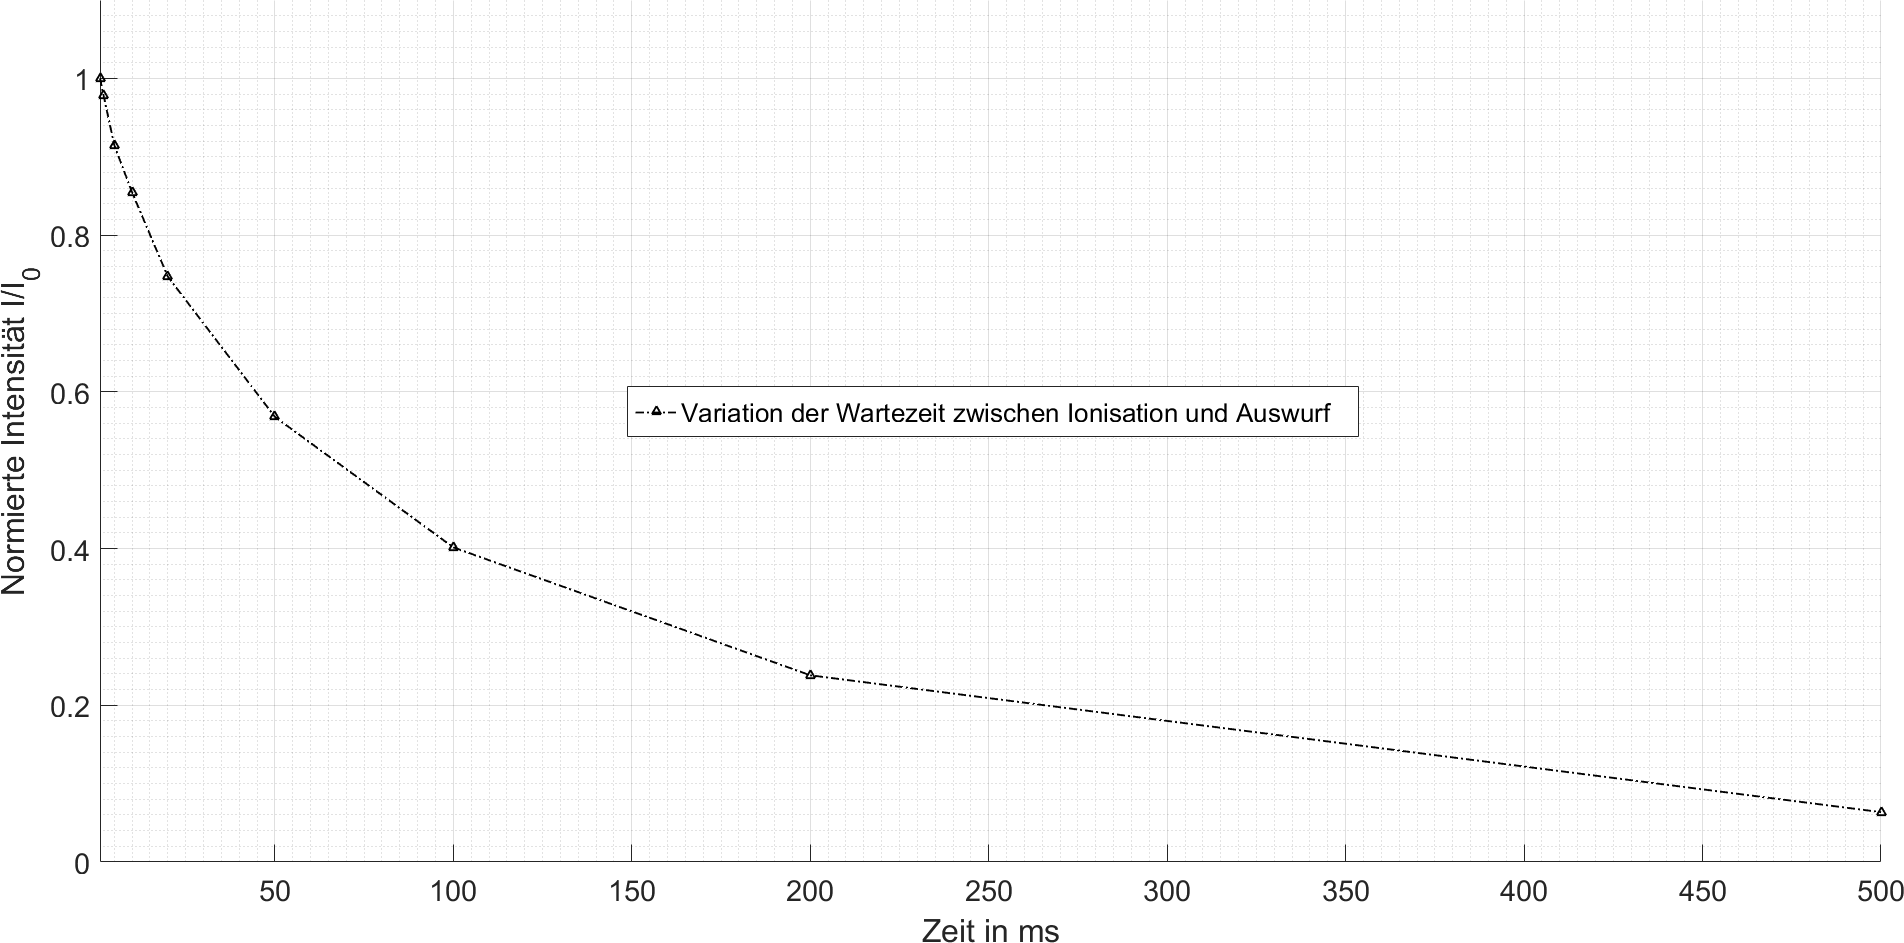
\includegraphics[width=\textwidth]{pics/wartezeit.png}
			\caption{Norm. Signalintensität über Variation der Wartezeit zwischen Ionisation und Auswurf auf den Detektor.}\label{img:zeit}
		\end{figure}
		
		\begin{figure}
			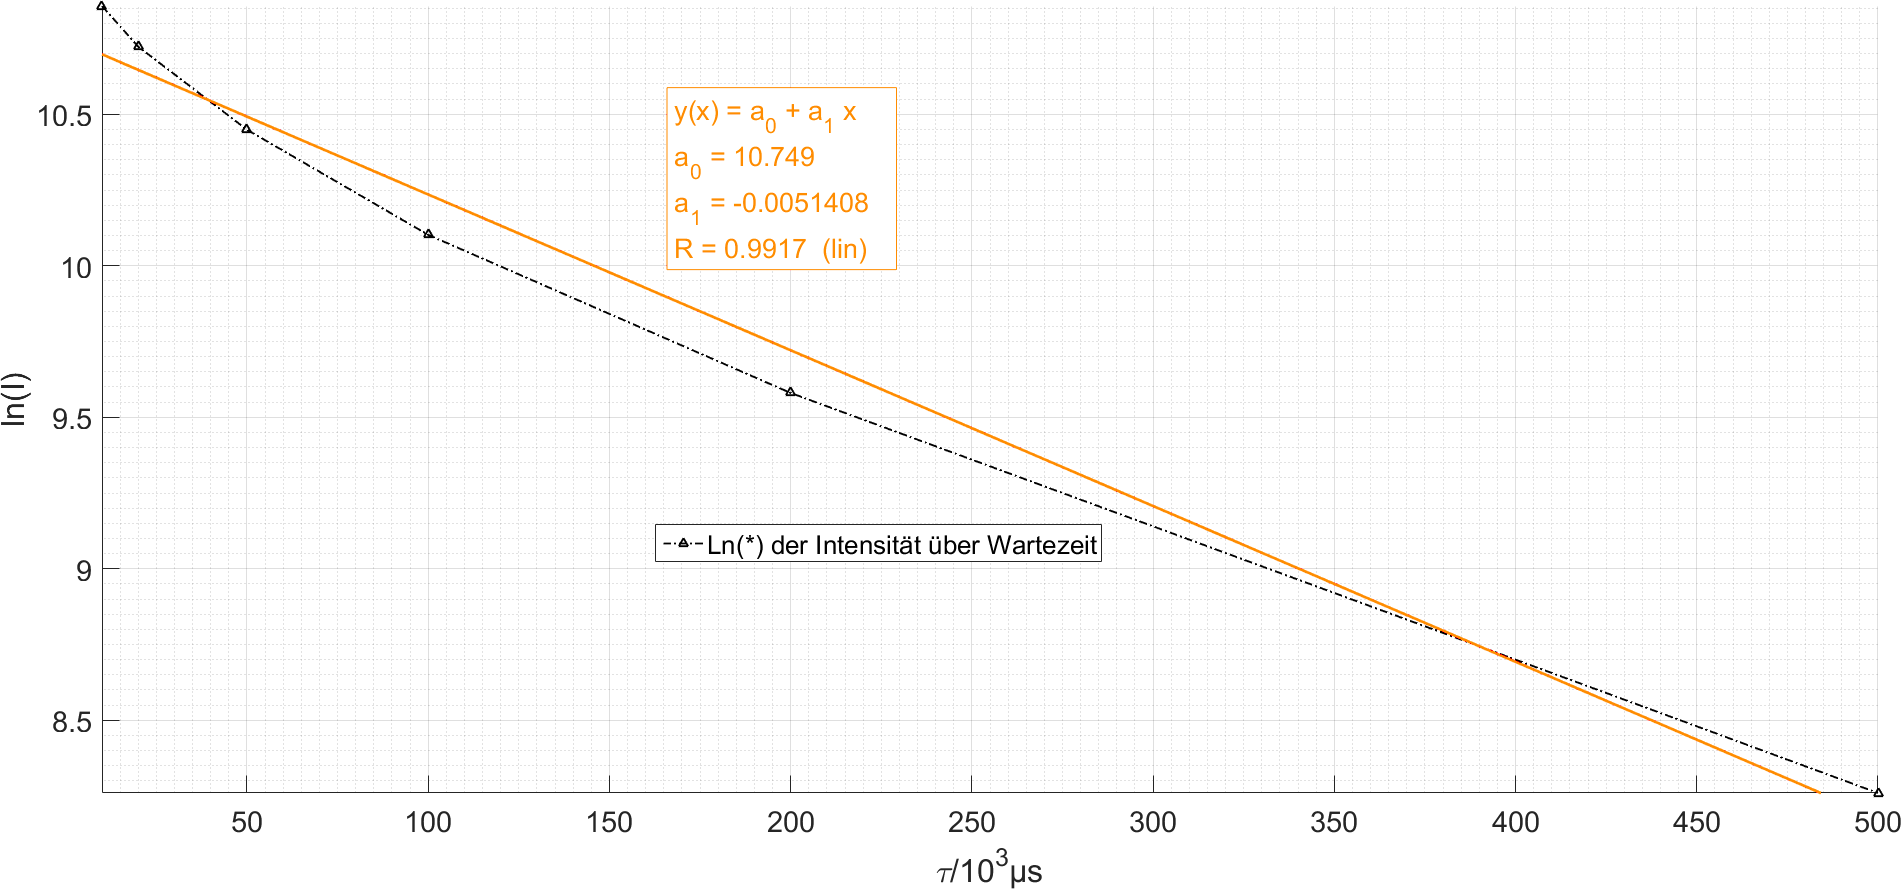
\includegraphics[width=\textwidth]{pics/linear_fit_wartezeit.png}
			\caption{Fit eines Polynoms erster Ordnung an den Logartihmus der Intensität. Die erhaltene Funktion ist eingezeichnet. Der Koeffizient $a_1$ gibt die Lebens- oder Speicherdauer in Fall wieder.}\label{img:lin}
		\end{figure}
		
		\subsection{Frequenzvariation der primären Anregung}
		
		In dieser Messung wurde die Frequenz der primären Anregung zum Auswurf aus der Falle auf den Detektor verändert. Es wurde das gleiche Mess- und Datenaufnahmeprinzip wie zuvor verwendet. Die Messparameter sind insbesondere die selben. In $\unit[10]{kHz}$-Schritten wurde ein Bereich von $\unit[\tenpo{5}]{Hz}$ bis $\unit[5\cdot\tenpo{5}]{Hz}$ abgerastert. Das Ergebnis zeigt \autoref{img:auswurf}. Damit sind des weiteren die bereits verwendeten Einstellungen der Manipulation bestätigt, da sich ein deutliches, unter anderem auch globales Maximum der Intensität des Ionenstromes auf den Detektor bei $\unit[350]{kHz}$ findet. Außerdem sind Nebenmaxima - bei ca. $\unit[110]{kHz}$, $\unit[140]{kHz}$ und $\unit[210]{kHz}$ - zu sehen, wie sie von den Vorbetrachtungen vorhergesagt wurden. Auf die Untersuchung dieser zielt die nächste Messung ab (siehe \autoref{subsec:mess}).
		
		\begin{figure}
			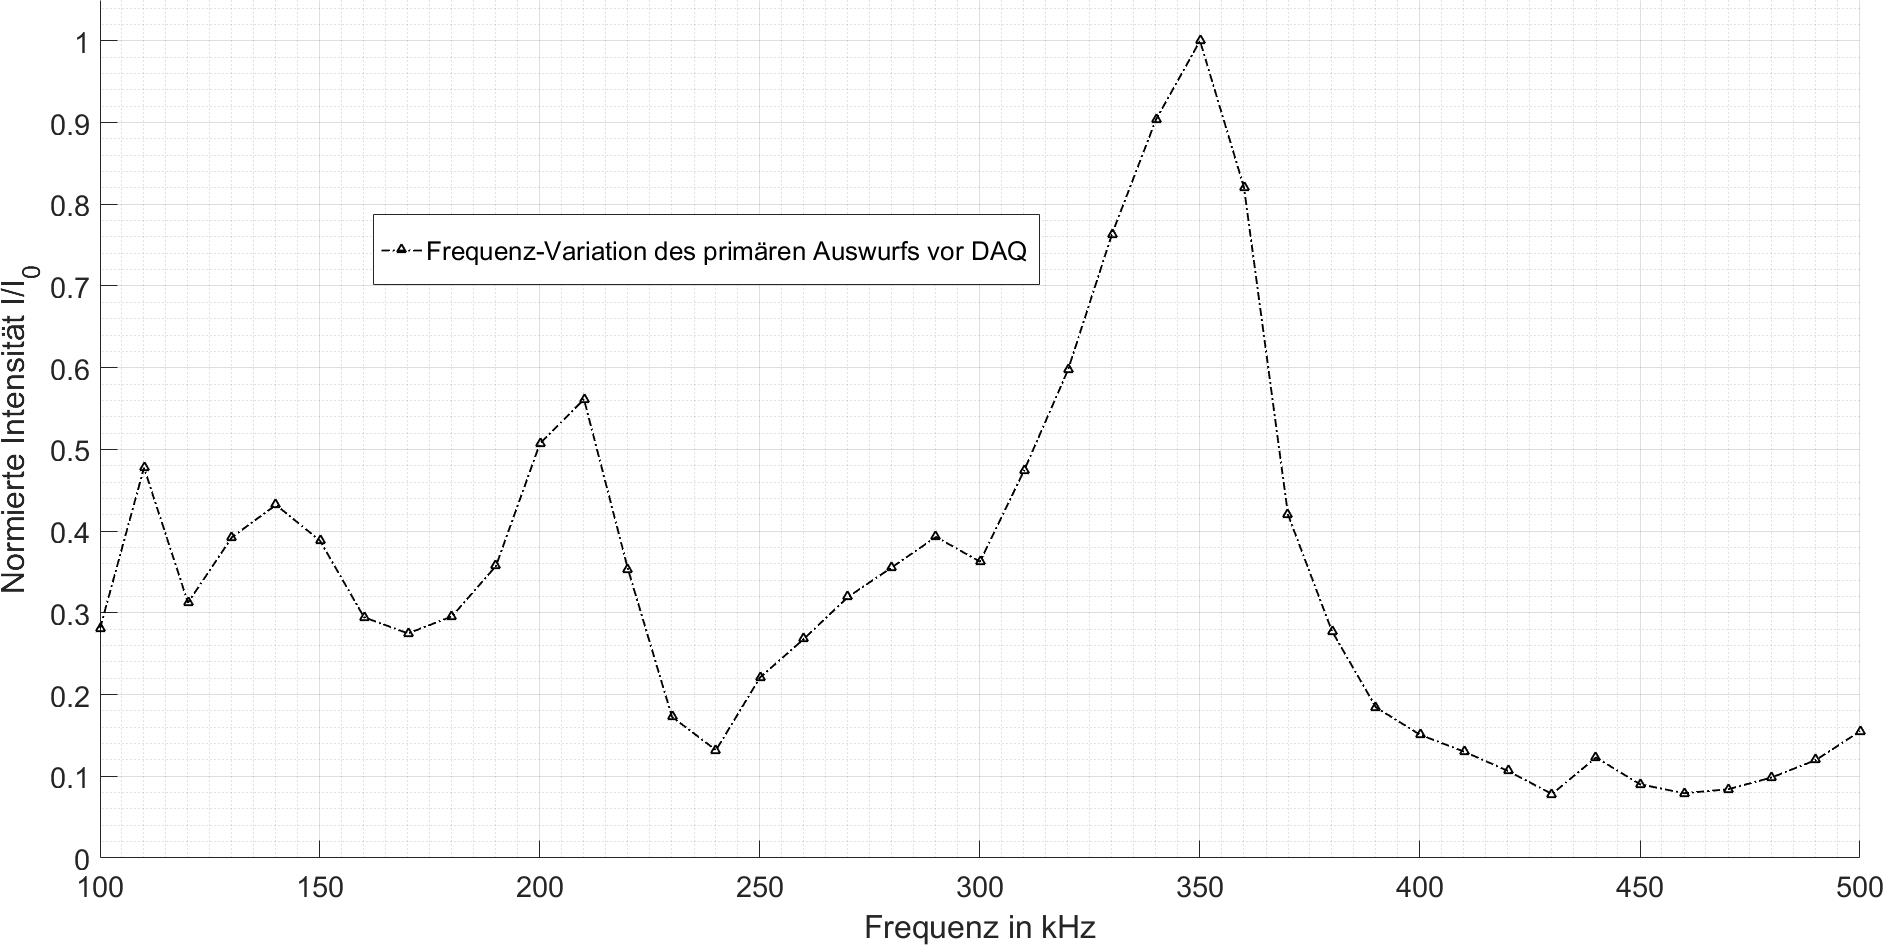
\includegraphics[width=\textwidth]{pics/freq_auswurf.png}
			\caption{Signalintensität als Funktion der Frequenz des primären Auswurfs vor der Datenaufnahme. Strukturen sind deutlich, welche die Überlegungen der Grundlagen bestätigen und die Wahl einer Auswurf-Frequenz von $\unit[350]{kHz}$ nahe legen.}\label{img:auswurf}
		\end{figure}
		
		\subsection{Untersuchung der Eigenfrequenzen von ionisiertem Stickstoff}\label{subsec:mess}
		
		Bei dieser Messung ist es wichtig, das vollständige Spektrum der Anregung zu betrachten, da viele Frequenzen und deren lineare Kombinationen darin eingehen. Deswegen wurde ein Intervall von 0 bis $\unit[1,5]{MHz}$ gewählt, da bei der Führungsfeldfrequenz und in dessen Umgebung eine verstärkte Dynamik zu erwarten ist.\\
		Ein einzelner Zyklus startet mit der Elektronenka none für 10000\,µs, worauf eine sekundäre Manipulation mit dem Frequenzschritt $f\ix{n}$ für 1000\,µs folgt. Danach 'ruht' die Messung für weitere 10000\,µs, wobei die Ionen einfach in der Falle verweilen. Schließlich läuft für 2000\,µs die Datenaufnahme des Detektors zusammen mit der primären Anregung mit $\unit[350]{kHz}$. Für jeweils einen solchen Zyklus gibt es einen Referenzverlauf, welcher im Anschluss dazu jedoch ohne die sekundäre Anregung erfolgt. Dieser dient der Eichung und Fehlerminderung. Das Ergebnis für 10 innere und 50 äußere Iterationen bei einer Schrittweite von $\unit[1]{kHz}$ zeigt \autoref{img:bullshit}.\\
		Ziel dieser Messung ist es, die Ionenintensität in Abhängigkeit von der Anregungsfrequenz aufzunehmen, um daraus ein Spektrum für die Eigenfrequenzen der Ionen zu erhalten. Man erwartet einen Verlauf nach dem Vorbild von \autoref{img:referenz}, wobei jedoch anderen Parameter verwendet wurden \cite{Paul-FalleREF}. Das Signal als Differenz von Referenz und sekundärer Anregung erhält demnach ein lokales Minimum, wenn mit einer Resonanzfrequenz der Probesubstanz angeregt wurde. Für den primären Auswurf auf den Detektor stehen dann weniger Ionen zur Verfügung.
		
		\begin{figure}
			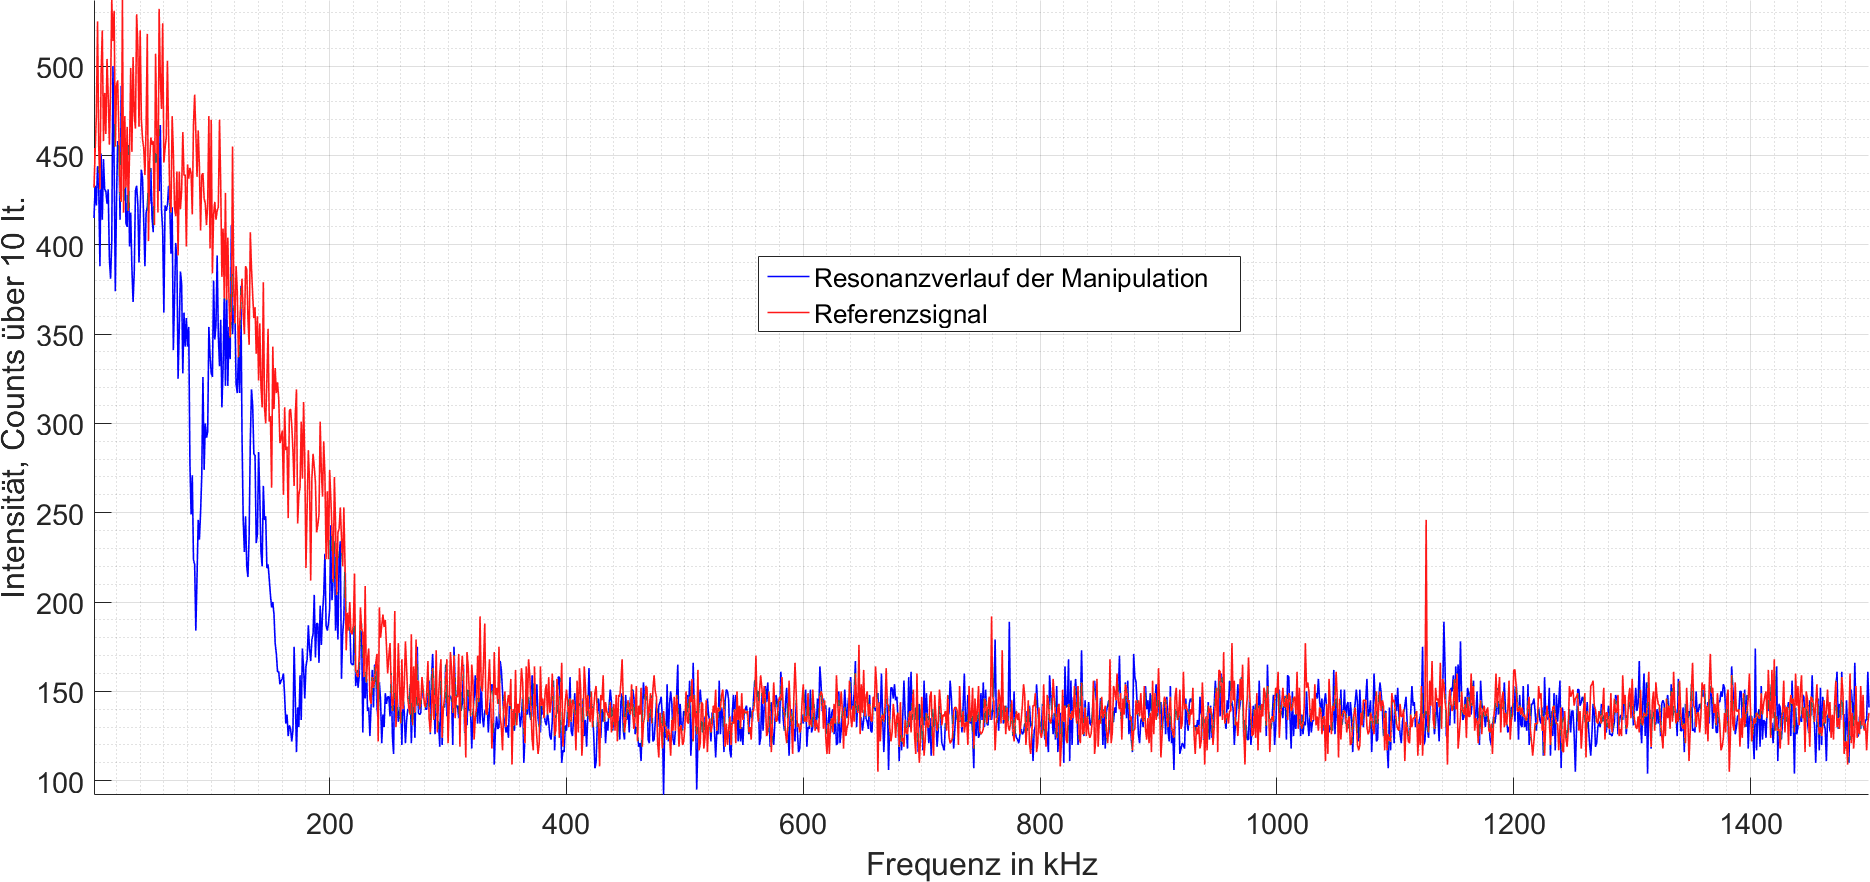
\includegraphics[width=\textwidth]{pics/volle_daten.png}
			\caption{Frequenziteration einer sekundären Anregung in $1\,kHz$-Schritten bis $1,5\,MHz$. Volles Spektrum der 50 aüßeren und 10 inneren Iterationen.}\label{img:bullshit}
		\end{figure}
		
		Die \autoref{img:resonanz} - und außerdem \autoref{img:1itsm} für die erste äußere Iteration bis $\unit[270]{kHz}$ - zeigt das letztendlich gesuchte Spektrum der Resonanzfrequenzen von $\fett{N}_2$-Ionen als die Differenz von Referenz- und Manipulationssignal.  Im Vergleich dazu ist der Verlauf aus \autoref{img:referenz} eingetragen, welcher für die selbe Ionensorte in \cite{Paul-FalleREF} aufgenommen wurde und hier als Literaturwert angenommen werden soll.\\
		Insgesamt scheint es so, als seien alle Resonanzen zu höheren Frequenzen verschoben worden. Angenommen dies sei der Fall, so wurden die Anregungen von $\omega_r$, $\omega_z$ und $\omega_z-\omega_r$ mit einem Fehler von $\pm\unit[20]{kHz}$ gefunden. Die ist aber insgesamt ein schwaches Kriterium, da bereits von einem Shift des gesamten Spektrums um etwa $+\unit[25]{kHz}$ auszugehen war. Eine Betrachtung der Fehler, welche konsequenter Weise aus dem Verlauf des Signals, insbesondere dem aus \autoref{img:bullshit} folgen, schließt sich im folgenden an.
		
		\begin{figure}
			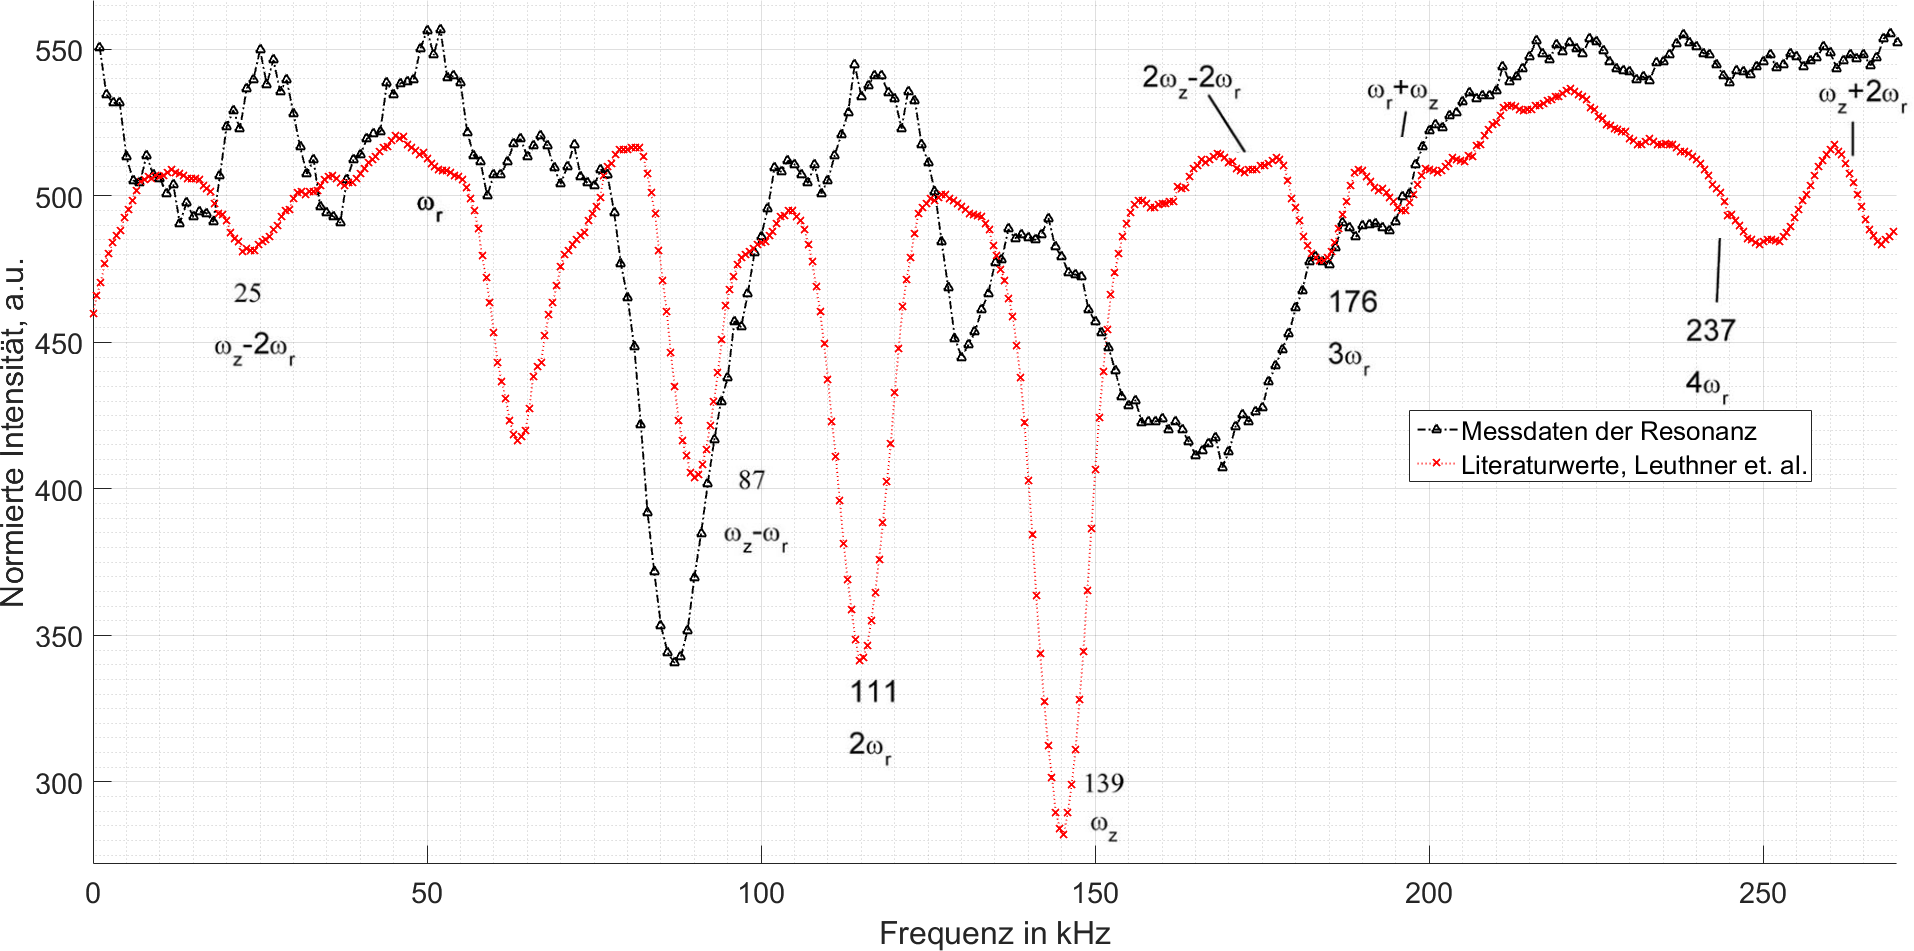
\includegraphics[width=\textwidth]{pics/freq_diff_vergleich.png}
			\caption{Differenz von Referenz und Manipulation. Vergleich mit der Literatur \cite{Paul-FalleREF} bei geringfügiger Übereinstimmung.}\label{img:resonanz}
		\end{figure}
		
		Die \autoref{img:bullshit} vermittelt außerdem ein indiskutables Problem: das Messsignal ist nach $\sim\unit[300]{kHz}$ quasi nicht mehr existent und wird von da an nur noch von der Nullzählrate oder anderen zufälligen Ereignissen bestimmt. Es liegt der Gedanke nahe, dass bei dieser großen Messdauer das Experiment nach einer bestimmen Aufnahmedauer versagt hat. Deshalb zeigt \autoref{img:1it} die erste äußere Iteration im vollen Spektrum  - und \autoref{limg:1itsm} - , woraus durch einen Vergleich der Intensitäten ersichtlich wird, das bereits dort die vollständigen Informationen der Messung enthalten sind.
		
		\begin{figure}
			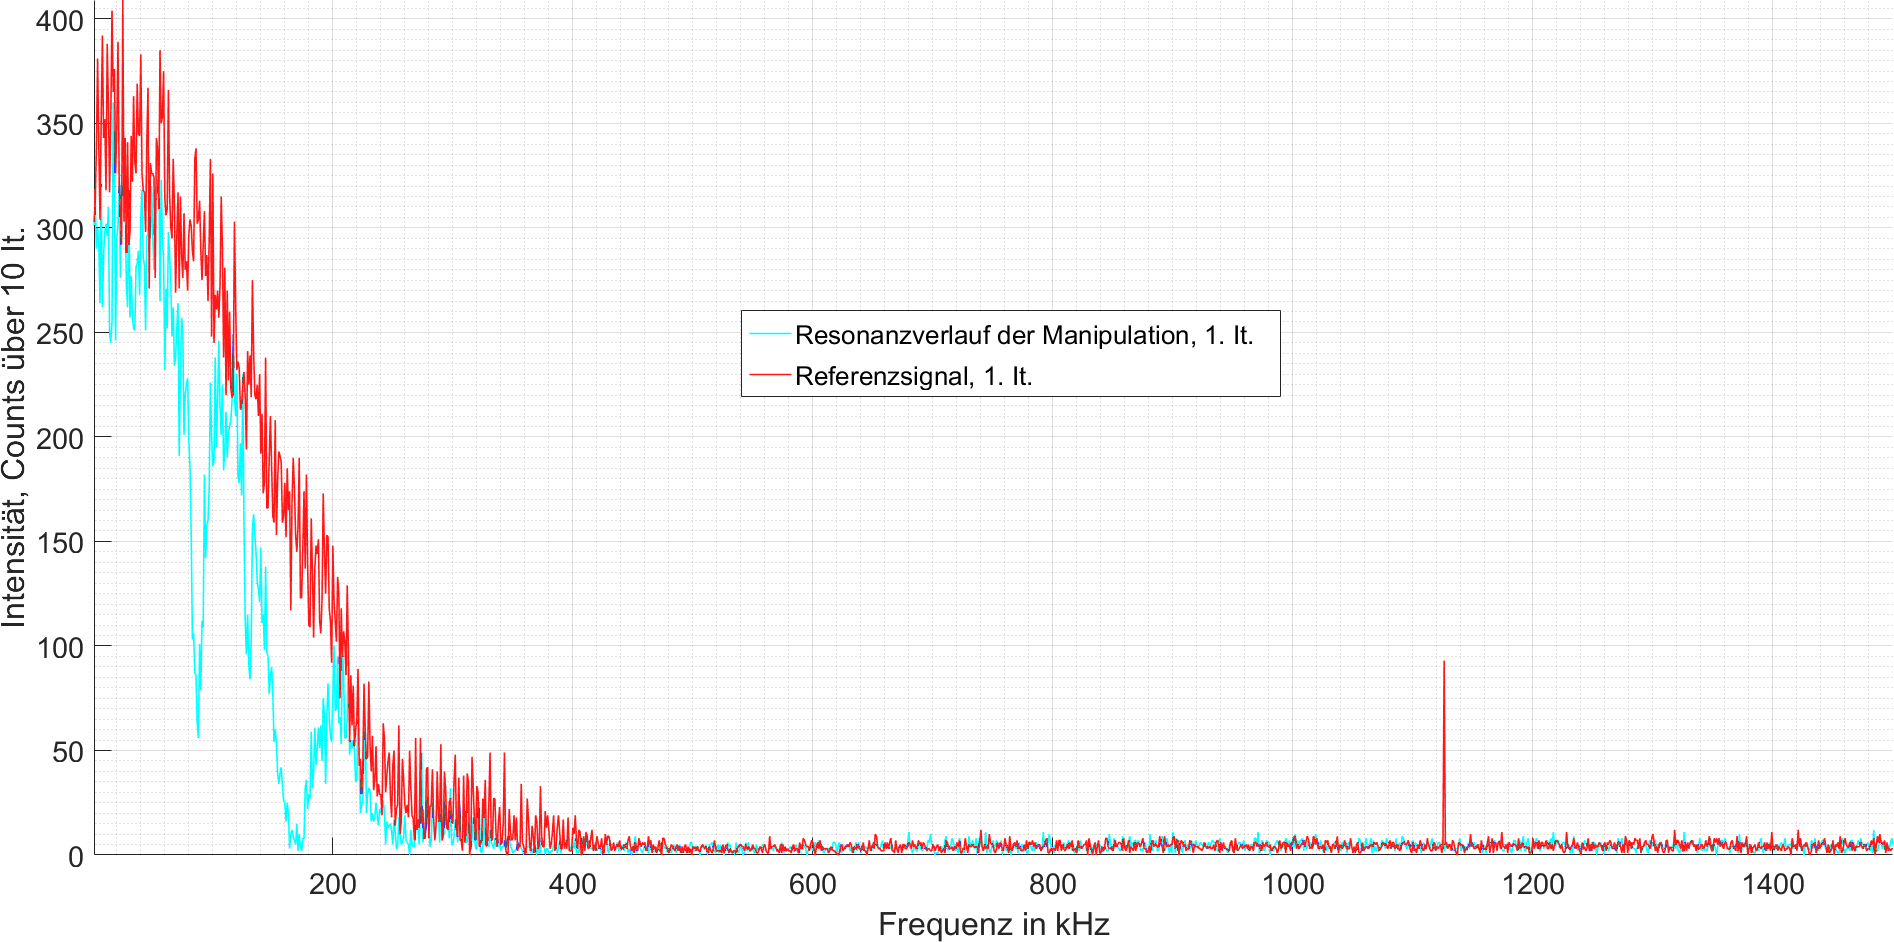
\includegraphics[width=\textwidth]{pics/erste_it.png}
			\caption{Signal der ersten Iteration. Im Vergleich zum Vollen Spektrum erkennt man leicht, das hier die vollständigen, erhaltenen Daten stecken.}\label{img:1it}
		\end{figure}
		
		\begin{figure}
			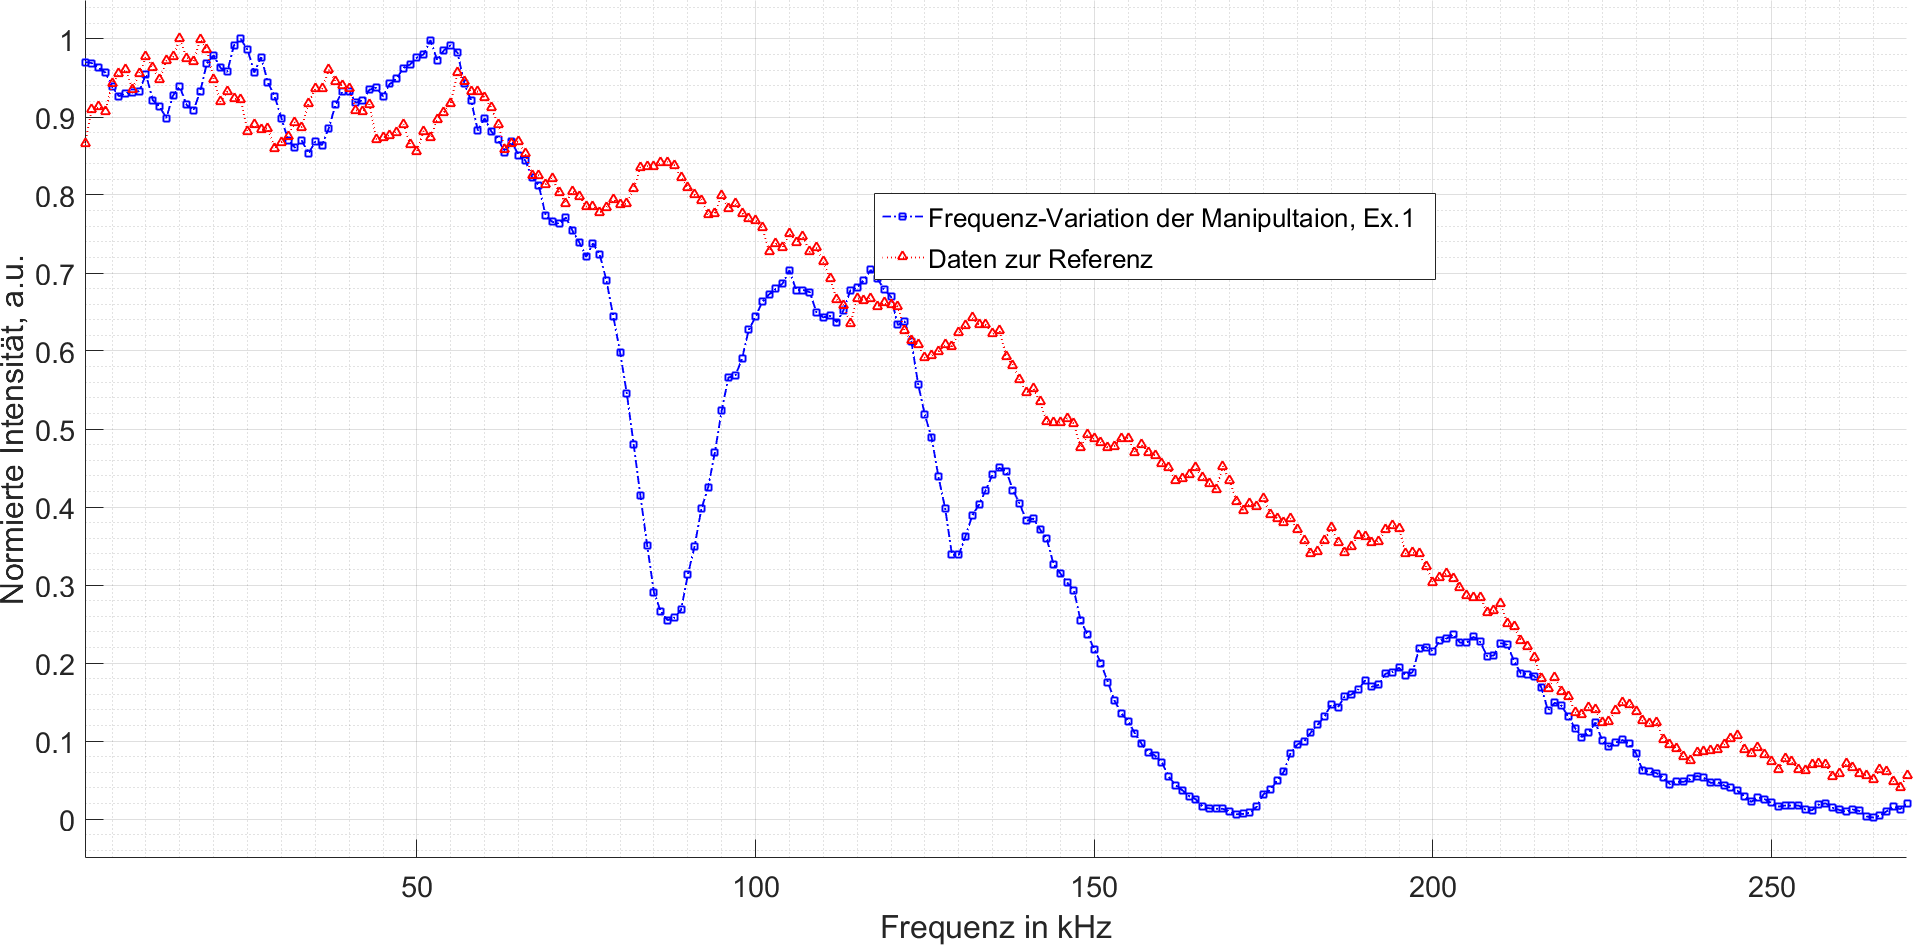
\includegraphics[width=\textwidth]{pics/freq_smooth.png}
			\caption{Abfall der Signalstärke in Referenz und Manipulation. Unbearbeitete Daten für \autoref{img:resonanz}.}\label{img:1itsm}
		\end{figure}
		
		Nach dieser ernüchternden Erkenntnis wurde versucht, das Problem des Signalverlusts zu erkennen und zu beheben. Dafür betrachtete man das verbliebene Signal über der Experiment-Dauer. Wieder stehen dabei ein Manipulations- und ein Referenz-Zyklus im Vergleich: 10000\,µs E-Kanone für Ionisation, 1000\,µs sekundäre Anregung bzw. Warten, 10000\,µs Warten und 20000\,µs primäre Anregung mit Auswurf und Datenaufnahme. Der signifikante Unterschied zu vorherigen Messungen ist die, bei beiden Verfahren eingeführte Verweildauer von 50000\,µs nach der Detektor-Aufnahme - sozusagen als Pause des Experimentes zwischen Messungen. Ziel dabei war es, den möglichen Einfluss von Aufladungseffekten auf den Bauteilen und Raumladungen in der Falle zu minimieren. Die \autoref{img:abnahme} zeigt das Resultat von 50 äußeren und 10 inneren Iterationen.\\
		Bei einer anfänglich, bereits außergewöhnlich niedrigen Intensität von $\unit[207]{Cnts./10 It.}$ fällt das Signal mit rund $\unit[2]{Cnts./1000\,ms}$ ab. Nicht aber, dass dies nur der Fall für die sekundäre Anregung wäre, sondern auch für das Signal der Referenzmessung. Dies zeigt an, dass ein konzeptionelles Problem mit dem Aufbau bzw. der Falle selbst vorliegen muss. Weitere Messungen ergaben sich als nicht aussagekräftig, da bei nachfolgenden Zyklen das Signal sogar noch schwächer wurde oder sogar in das statistische Rauschen aus \autoref{img:bullshit} über ging. Im Rahmen dieses Praktikums und eines einzelnen Versuches über 2 Tage war es uns leider nicht möglich, tiefer greifende Fehleranalysen und Problembehebungen für die vorgestellten Hindernisse durchzuführen.
		
		\begin{figure}
			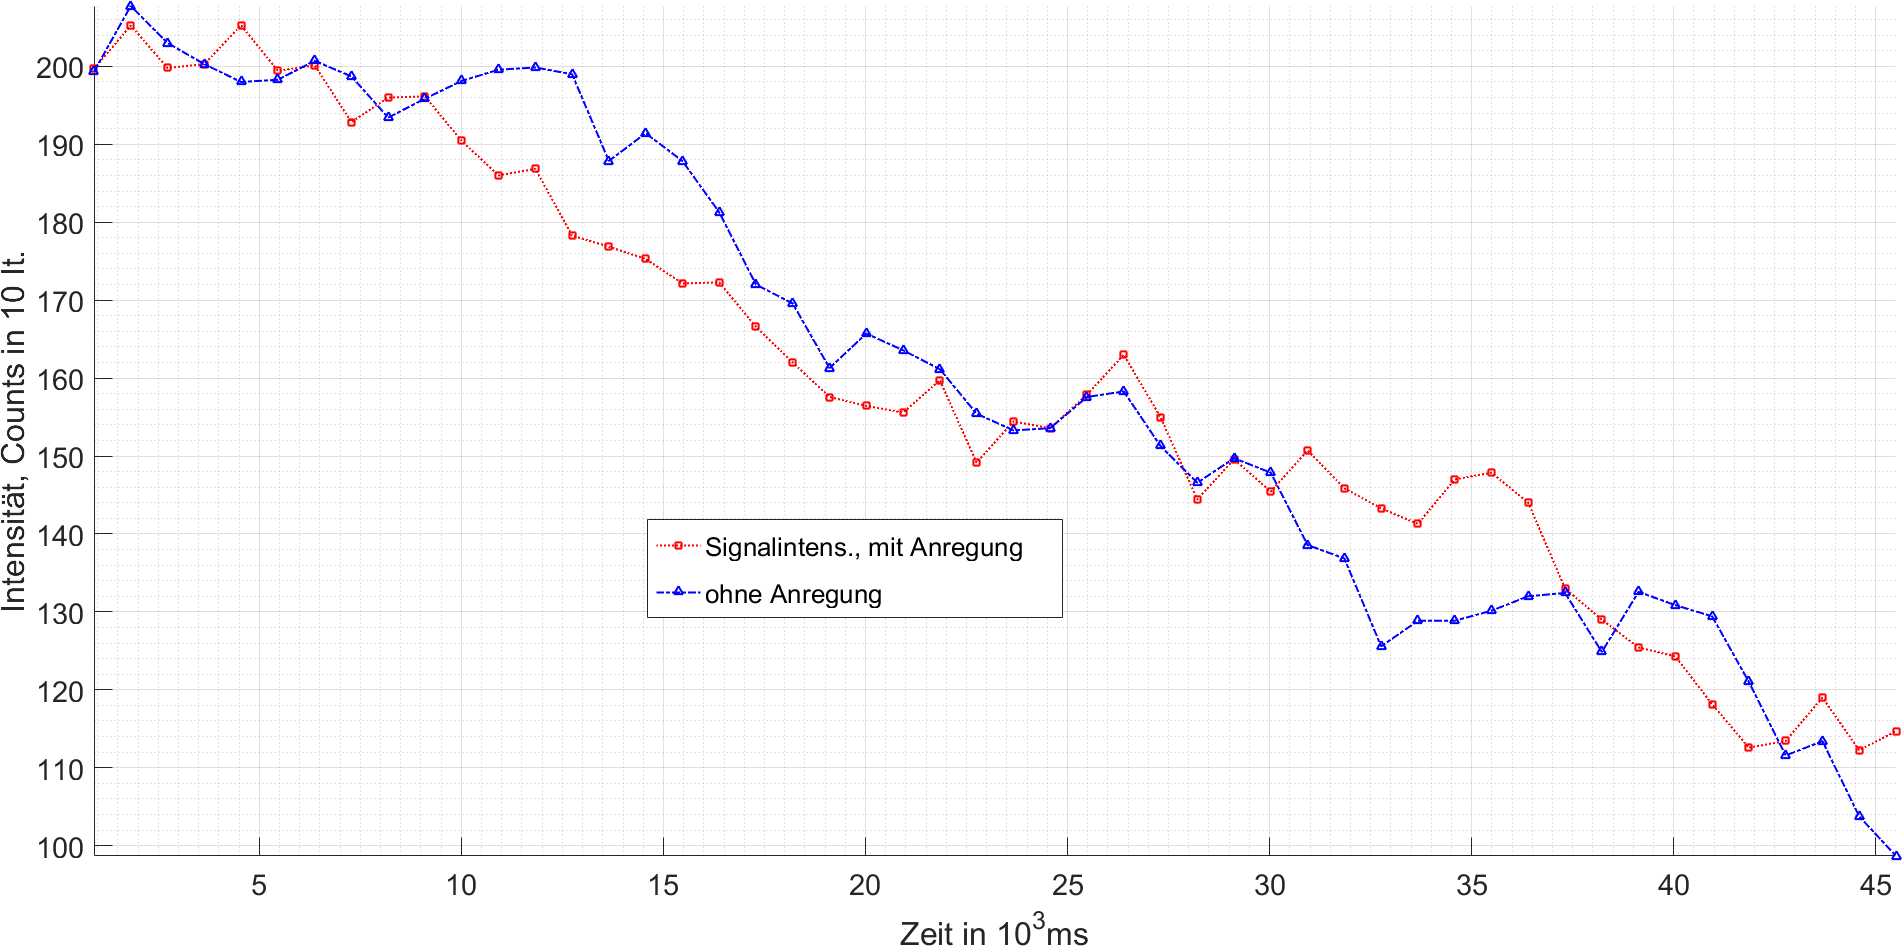
\includegraphics[width=\textwidth]{pics/signal_abfall.png}
			\caption{Untersuchung des Intensitäts-Abfalls über der Experimentdauer. Sehr geringen Signalstärken gegenüber den Intensitäten aus \autoref{img:zeit}, welche im Bereich bon 5000-10000 lagen (dort nur normiert).}\label{img:abnahme}
		\end{figure}
		
		\clearpage
		\section{Anhang}
		
		\bibliography{all.bib}
		\bibliographystyle{unsrt}
		
	\end{document}